\documentclass[crop, tikz]{standalone}
\usepackage{tikz}

\usetikzlibrary{snakes}

\definecolor{mygreen}{HTML}{006400}
\definecolor{mymauve}{rgb}{0.58,0,0.82}
\definecolor{mygold}{HTML}{B8860B}
\definecolor{mynavy}{HTML}{000080}

\begin{document}
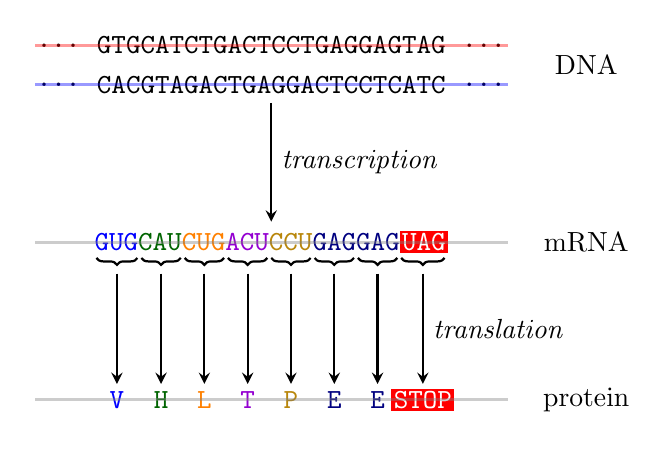
\begin{tikzpicture}
	\node at (0,0) {\tt GTGCATCTGACTCCTGAGGAGTAG};
	\node (dnk2) at (0,-0.5) {\tt CACGTAGACTGAGGACTCCTCATC};
	\node at (-2.7, 0) {\tt \dots};
	\node at (2.7, 0) {\tt \dots};
	\node at (-2.7, -0.5) {\tt \dots};
	\node at (2.7, -0.5) {\tt \dots};
	\draw[red, opacity=0.4, very thick] (-3, 0) -- (3, 0);
	\draw[blue, opacity=0.4, very thick] (-3, -0.5) -- (3, -0.5);
		
	\node at (4, -0.25) {DNA};
		
	\node (rnk) at (0,-2.5) {\tt \textcolor{blue}{GUG}\textcolor{mygreen}{CAU}\textcolor{orange}{CUG}\textcolor{mymauve}{ACU}\textcolor{mygold}{CCU}\textcolor{mynavy}{GAGGAG}\tikz[baseline]{\node[rectangle, fill=red,inner sep=0.3mm,anchor=base] (X) {\textcolor{white}{UAG}};}};
	\draw[gray, opacity=0.4, very thick] (-3, -2.5) -- (3, -2.5);
		
	\draw [thick, decoration={ brace, mirror, raise=0.5cm}, decorate] (-2.22, -2.2) -- (-1.7, -2.2); 
	\draw [thick, decoration={ brace, mirror, raise=0.5cm}, decorate] (-1.65, -2.2) -- (-1.15, -2.2); 
	\draw [thick, decoration={ brace, mirror, raise=0.5cm}, decorate] (-1.1, -2.2) -- (-0.6, -2.2); 
	\draw [thick, decoration={ brace, mirror, raise=0.5cm}, decorate] (-0.55, -2.2) -- (-0.05, -2.2); 
	\draw [thick, decoration={ brace, mirror, raise=0.5cm}, decorate] (0, -2.2) -- (0.5, -2.2); 
	\draw [thick, decoration={ brace, mirror, raise=0.5cm}, decorate] (0.55, -2.2) -- (1.05, -2.2); 
	\draw [thick, decoration={ brace, mirror, raise=0.5cm}, decorate] (1.1, -2.2) -- (1.6, -2.2); 
	\draw [thick, decoration={ brace, mirror, raise=0.5cm}, decorate] (1.65, -2.2) -- (2.2, -2.2); 
		
	\node at (4, -2.5) {mRNA};
		
	\draw[-stealth, thick] (dnk2) -- node[right] {\emph{transcription}} (rnk);
		
	\draw[-stealth, thick] (-1.96, -2.9) -- (-1.96, -4.3);
	\node at (-1.96, -4.5) {\tt \textcolor{blue}V};
		
	\draw[-stealth, thick] (-1.4, -2.9) -- (-1.4, -4.3);
	\node at (-1.4, -4.5) {\tt \textcolor{mygreen}H};
		
	\draw[-stealth, thick] (-0.85, -2.9) -- (-0.85, -4.3);
	\node at (-0.85, -4.5) {\tt \textcolor{orange}L};
		
	\draw[-stealth, thick] (-0.3, -2.9) -- (-0.3, -4.3);
	\node at (-0.3, -4.5) {\tt \textcolor{mymauve}T};
		
	\draw[-stealth, thick] (0.25, -2.9) -- (0.25, -4.3);
	\node at (0.25, -4.5) {\tt \textcolor{mygold}P};
	
	\draw[-stealth, thick] (0.8, -2.9) -- (0.8, -4.3);
	\node at (0.8, -4.5) {\tt \textcolor{mynavy}E};
		
	\draw[-stealth, thick] (1.35, -2.9) -- (1.35, -4.3);
	\node at (1.35, -4.5) {\tt \textcolor{mynavy}E};
		
	\draw[-stealth, thick] (1.925, -2.9) -- node[right] {\emph{translation}} (1.925, -4.3);
	\node at (1.925, -4.5) {\tikz[baseline]{\node[rectangle, fill=red,inner sep=0.3mm,anchor=base] (X) {\textcolor{white}{\tt STOP}};}};
		
	\draw[gray, opacity=0.4, very thick] (-3, -4.5) -- (3, -4.5);
		
	\node at (4, -4.5) {protein};
\end{tikzpicture}	
\end{document}
